\documentclass[twocolumn, fontsize=10pt]{article}
\usepackage{xeCJK}
\usepackage[margin=0.70in]{geometry}
\usepackage{lipsum,mwe,abstract}
\usepackage[T1]{fontenc} 
% \usepackage[english]{babel} 

\usepackage{fancyhdr} % Custom headers and footers
\pagestyle{fancyplain} % Makes all pages in the document conform to the custom headers and footers
\fancyhead{} 
\fancyfoot[C]{\thepage} % Page numbering for right footer
\usepackage{lipsum}
\setlength\parindent{0pt} 
\usepackage{amsmath,amsfonts,amsthm} % Math packages
\usepackage{wrapfig}
\usepackage{caption}
\usepackage{subcaption}
\usepackage{graphicx}
\usepackage{float}
\usepackage{tablefootnote}
\usepackage{subcaption}
\usepackage{booktabs}
\usepackage{makecell}
\usepackage[title]{appendix}
\usepackage{comment}
\usepackage{minted}
\usepackage{enumitem}
\usepackage[colorlinks,linkcolor=black,anchorcolor=blue]{hyperref}
\usepackage{cuted}
\usepackage{dblfloatfix}
\usepackage{sectsty} % Allows customizing section commands
\allsectionsfont{\normalfont \normalsize \scshape} % Section names in small caps and normal fonts

\setlength{\parskip}{0.5em}

\linespread{1.1}

\XeTeXlinebreaklocale "zh" %文字間隔

\XeTeXlinebreakskip = 0pt plus 1pt

\renewenvironment{abstract} % Change how the abstract look to remove margins
 {\small
  \begin{center}
  \bfseries 摘要\vspace{-.5em}\vspace{0pt}
  \end{center}
  \list{}{%
    \setlength{\leftmargin}{0mm}
    \setlength{\rightmargin}{\leftmargin}%
  }
  \item\relax}
 {\endlist}
 
\makeatletter
\renewcommand{\maketitle}{\bgroup\setlength{\parindent}{0pt} % Change how the title looks like
\begin{flushleft}
  \textbf{\@title}
  \@author \\ 
  \@date
\end{flushleft}\egroup
}
\makeatother

%% ------------------------------------------------------------------- 

\captionsetup[figure]{labelfont={bf},labelformat={default},labelsep=period,name={图}}
\captionsetup[table]{labelfont={bf},labelformat={default},labelsep=period,name={表}}
\renewcommand{\refname}{参考文献}
\renewcommand{\contentsname}{目录}
\renewcommand{\appendixname}{附录}


\title{
\Large 基于卷积神经网络的糖尿病视网膜病变分类网络\\ \vspace{0.5em}
}
\date{}
\author{\, 网络空间安全学院\quad 信息安全、法学\quad 2111876\quad 梅骏逸}

\begin{document}

\twocolumn[ \maketitle ]

% --------------- ABSTRACT
\begin{abstract}
      糖尿病视网膜病变分级问题由于数据集不平衡等问题一直作为一个困难的分类问题存在。本实验基于卷积神经网络,结合预训练模型以及多种特征提取的卷积网络实现了对糖尿病视网膜病变的分级,并且在 DDR 数据集上进行了测试和对比,取得了不错的效果。
\end{abstract}

{\small\textbf{关键词:} 预训练;卷积神经网络;分类}

\rule{\linewidth}{0.7pt}

\tableofcontents

\section{导言}
  糖尿病视网膜病变分级(Diabetic Retinopathy Grading)由于存在样本不均衡等问题,对于基于深度学习的分类器来说存在着挑战。而对于 DDR 数据集\cite{LI2019},其样本不均衡的问题也仍然存在(如图 \ref{fig:data_dist} 所示)。

\begin{figure}
    \centering
    \includegraphics[width=7cm]{data_dist.pdf}
    \caption{DDR 数据集中不同类别数据的比例}
    \label{fig:data_dist}
\end{figure}

  本实验采用了添加预训练模型、加入 Label Smoothing 方法进行了实验,尝试减少样本不均衡问题带来的对模型的影响,并且在测试集取得了较好的效果\footnote{本实验的有关代码可以在仓库 \url{https://github.com/JuniMay/diabetic-retinopathy-classification} 中找到。}。

\section{使用的模型}

  模型首先使用一个 Backbone 作为特征提取器对输入的图片进行处理,Backbone 采用了现有的一些预训练的卷积网络模型,同时也尝试了使用 Patch Embedding 的方式进行处理。经过 Backbone 的处理之后得到的特征,通过一个 CBAM \cite{woo2018}注意力机制模块,之后进入一系列的 ConvMixer 模块中处理。

  ConvMixer\cite{trockman2022} 是一个较为精简的卷积网络模型,其最基本的模块 ConvMixer Block 将输入的内容经过一次 Depthwise 卷积之后,通过 GELU 激活函数处理和批标准化处理之后进行一次残差连接。再进行一次 Pointwise 卷积,通过 GELU 激活并进行批标准化。ConvMixer 模块中的 Depthwise 和 Pointwise 卷积可以视作将一次卷积分成两次进行,第一次对每个通道使用不同的核进行卷积(Depthwise),第二次则在每一点上进行卷积(Pointwise),过程大致如图 \ref{fig:depth_point_wise_conv} 所示。
\begin{figure}
    \centering
    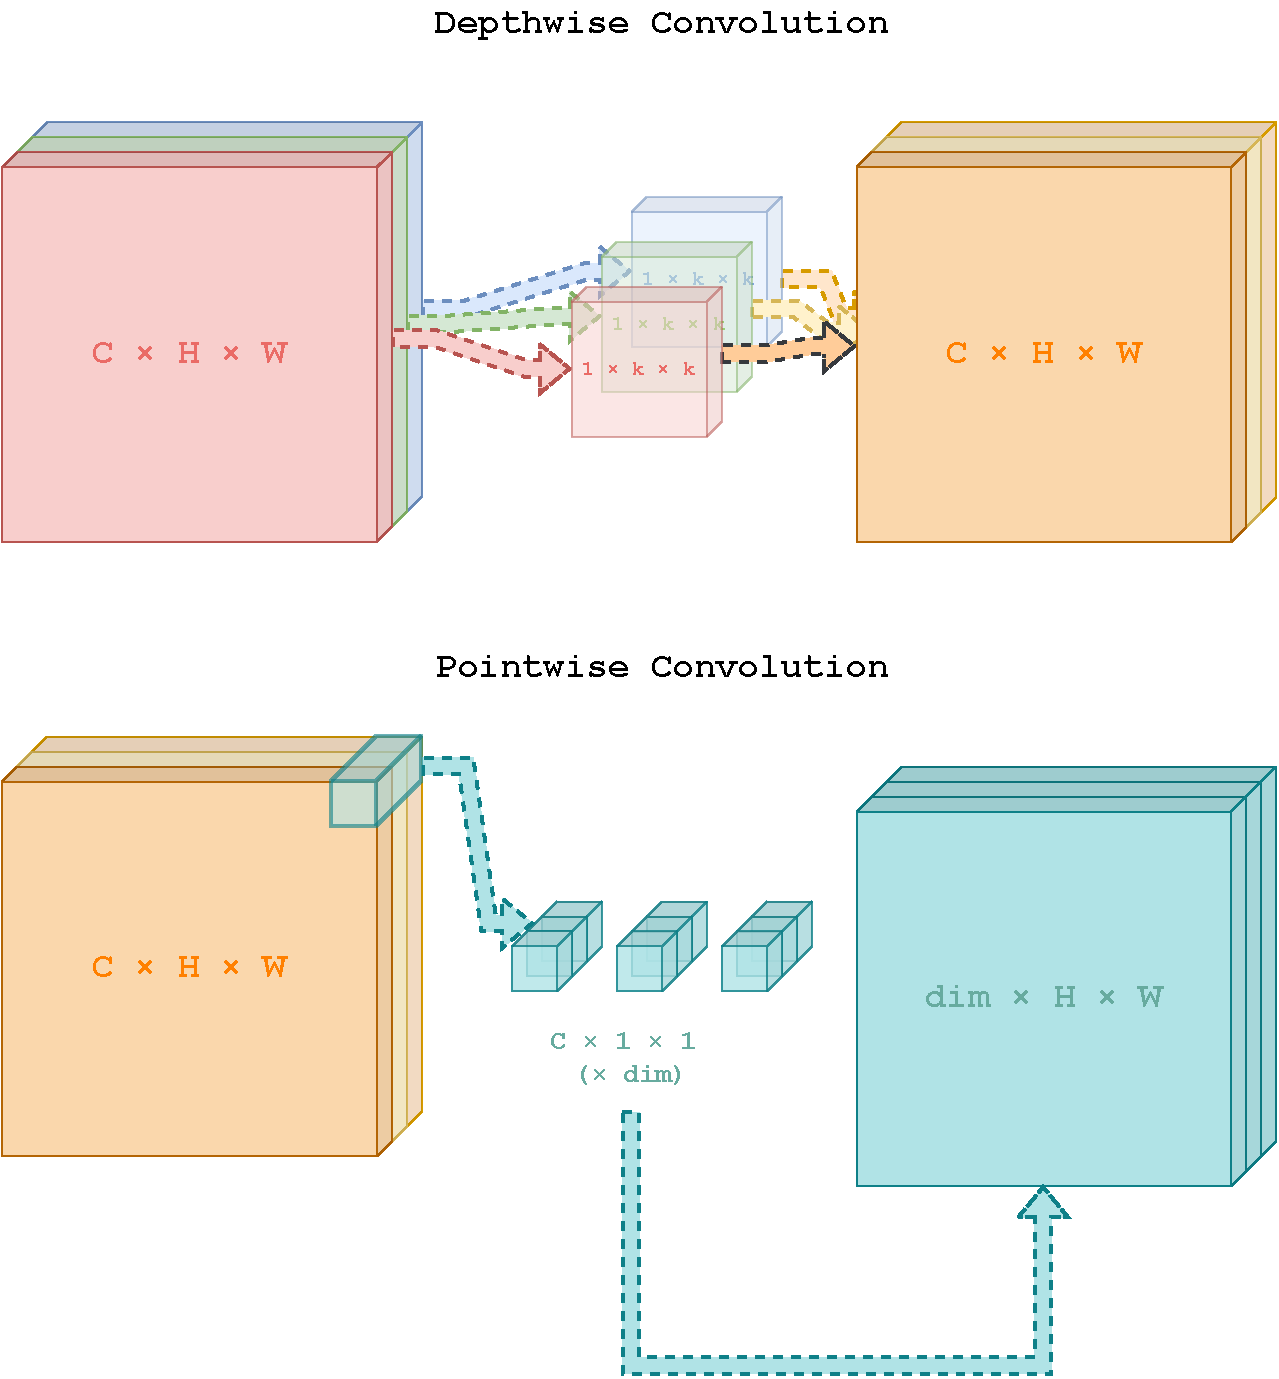
\includegraphics[width=7cm]{depth_point_wise_conv.pdf}
    \caption{Depthwise 及 Pointwise 卷积示意图}
    \label{fig:depth_point_wise_conv}
\end{figure}

  ConvMixer 模块处理之后的特征通过 Global Average Pooling\cite{lin2013} 进行池化并在降维之后使用一个全连接层进行分类。模型的完整结构如图 \ref{fig:model_structure} 所示。
\begin{figure}[h]
    \centering
    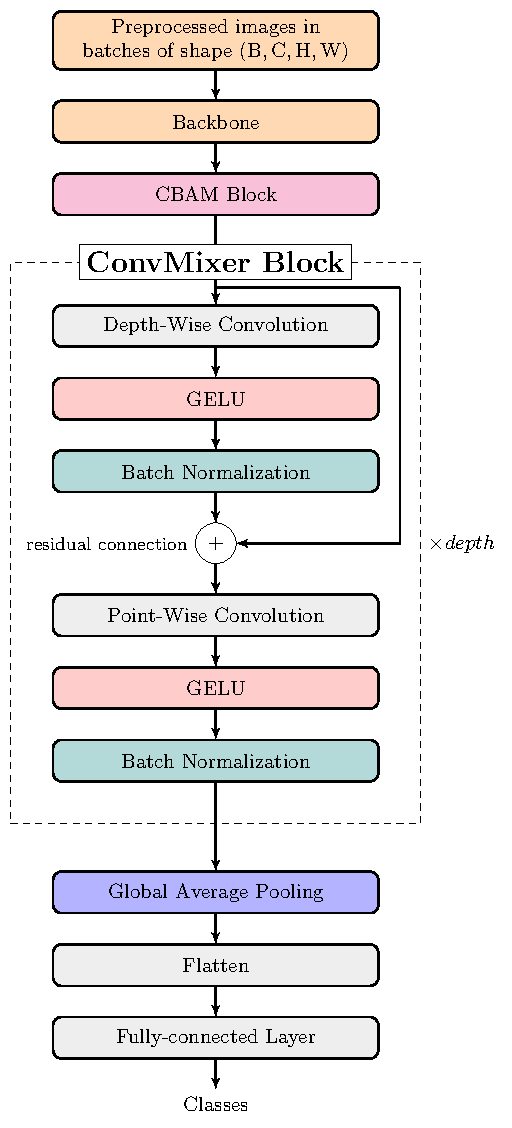
\includegraphics[width=6cm]{model.pdf}
    \caption{模型架构}
    \label{fig:model_structure}
\end{figure}

  除此之外,还对 CABNet\cite{he2021} 进行了实验对比。

\subsection{使用的特征提取器(Backbone)}

\subsubsection{Patch Embedding}

  使用 Patch Embedding 的方法从图片中提取特征参考了原始 ConvMixer 网络所采用的方法。其作用在于将原始的图像通过卷积的方式进行分块,以大小为 $p$ 的 Patch 做 Patch Embedding 操作即为以 $p$ 为卷积的步长(stride)以 $p$ 为核的大小(kernel size) 对输入做卷积。

  ConvMixer 原始网络\cite{trockman2022}中的 Patch Embedding 在做完分块的卷积之后进行了一次激活以及批标准化(Batch Normalization),实验中使用与之相同的方法实现 Patch Embedding,使用 GELU 作为激活函数。实现方式如下:
\begin{minted}[breaklines]{python}
class PatchEmbedding(nn.Module):
    def __init__(self, dim, patch_size, in_channels=3):
        super().__init__()
        self.conv = nn.Conv2d(in_channels, dim, patch_size, patch_size)
        self.activation = nn.GELU()
        self.norm = nn.BatchNorm2d(dim)

    def forward(self, x: torch.Tensor) -> torch.Tensor:
        x = self.conv(x)
        x = self.activation(x)
        x = self.norm(x)
        return x
\end{minted}


\subsubsection{预训练网络}

  除了 ConvMixer 论文中所使用的 Patch Embedding 方法,实验中还尝试了一些进行过预训练的现有卷积网络的一部分作为 Backbone,并将输出输入到后续处理中。

  ConvNeXt 通过采用过去各种卷积网络中的经验,使用 Patch、逆瓶颈层、GELU 激活函数并减少激活函数数量、减少标准化数量、使用 Layer Normalization 等方式在 ImageNet-1k 数据集上达到了不错的效果\cite{liu2022}。由于 ConvNeXt 所取得的优秀结果,在实验中共采取了三种方法使用 ConvNeXt 模型:
  \begin{enumerate}
      \item 将其参数冻结,将输出进入后续网络进行训练。
      \item 不冻结参数,改变全连接层一起训练
      \item 不冻结参数,将其输出输入到后续网络进行训练并且采用不一样的学习率。
  \end{enumerate}
所使用的这几种训练方法的具体结果见后文中的实验数据。ConvNeXt 的论文中具有几种不同的参数组合,此处处于计算量、算力和时间的考量使用了 ConvNeXt-Base,并使用 torchvision 内置的模块导入原始网络。

  在 ConvNeXt 之外,实验中还使用了 EfficientNet\cite{tan2019} 和 DenseNet\cite{huang2016} 作为 Backbone 进行尝试。DenseNet 主要机制是将每一层的输出接(Concatenate)起来作为下一层输入,EfficientNet 的优势则在于较小参数量和较快的速度。实验中使用了 DenseNet-121 和 EfficientNet-B4 作为 Backbone,不冻结参数并与后续网络设置不同的学习率。

\subsection{注意力模块}

  在 Backbone 之后是一个卷积注意力模块(Convolutional Block Attention Module, CBAM)\cite{woo2018},CBAM 模块的机制大致可以表示如下:
$$
\begin{aligned}
    w_1 &=\sigma(\mathsf{MLP}(\mathsf{AvgPool}(x_0))+ \mathsf{MLP}(\mathsf{MaxPool}(x_0)))\\
    x_1 &= w_1 \otimes x_0\\
    w_2 &=\sigma(\mathsf{Conv}_{2\rightarrow 1}([\mathsf{AvgPool}(x_1); \mathsf{MaxPool}(x_1)]_{\mathsf{concat}}))\\
    x_2 &= w_2 \otimes x_1
\end{aligned}
$$
即用一个相同的 MLP 对 AvgPool 和 MaxPool 之后的输入进行操作并相加,经过 sigmoid 激活之后作为对应通道的权重乘上原始数据(对应相乘),将得到的 $x_1$ 的 AvgPool 和 MaxPool 在通道的维度上连接(Concatenate)起来,并进行卷积(通道数从 2 至 1),最后通过激活函数作为对应元素的权重与 $x_1$ 相乘(对应相乘),得到的 $x_2$ 即为 CBAM 模块的输出。

\subsection{CABNET 网络结构}

  由于 CABNet\cite{he2021} 中的 Global Attention 和 Category Attention 在 DDR 数据集上的优秀表现,实验中还对 CABNet 使用 ConvNeXt 网络作为 backbone 进行了实验\footnote{实验中使用 PyTorch 实现 CABNet,实现中网络的结构与论文中所描述的一致。}。

  Global Attention 与 CBAM 类似,由通道注意力与空间注意力组成,但是在实现的方式上存在差别。通道注意力首先通过池化、卷积、激活得到通道权重并与输入相乘。之后在通道的维度上进行平均池化、激活得到权重并相乘,其过程可形式化为如下表达式:

$$
\begin{aligned}
w_1 &=\sigma(\mathsf{Conv}(\mathsf{AvgPool}(x_0)))\\
x_1 &= w_1 \otimes x_0\\
w_2 &=\sigma(\mathsf{AvgPool_{channel}}(x_1))\\
x_2 &= w_2 \otimes x_1
\end{aligned}
$$

  在 Global Attention 之后引入一个 Category Attention 模块,将通道数增广到 $k\times L$,其中 $L$ 表示类别数量,通过池化得到每一类的权重;并在改变维数后对 $k$ 所在维度池化,将两种操作结果对应元素相乘并在通道维数上池化得到权重,与 Global Attention 的结果相乘得到结果,最后通过池化、Flatten 和全连接层得到分类结果。实验中根据 CABNet 论文中的实验结果,取 $k=5$。

\section{实验}


\begin{table*}[h!]
    \centering
    \begin{tabular}{lclclllc}
        \toprule
        Backbone        & Parameters     & Classification Net & Depth & Accuracy        & Kappa           & Image          & Batch Size \\
        \midrule
        Patch-Embedding & not pretrained & CBAM + ConvMixer   & 8     & 0.6911          & 0.4618          & 480$\times$480 & 128        \\
        ConvNeXt        & unfreezed      & FC                 & 8     & \textbf{0.8399} & 0.\textbf{7227} & 480$\times$480 & 32         \\
        ConvNeXt        & unfreezed      & CBAM + ConvMixer   & 4     & \textbf{0.8399} & 0.7218          & 480$\times$480 & 32         \\
        ConvNeXt        & unfreezed      & GAB + CAB          & -     &  0.8284         & 0.7001          & 480$\times$480 & 32         \\
        ConvNeXt        & freezed        & CBAM + ConvMixer   & 8     & 0.7526          & 0.5599          & 480$\times$480 & 128        \\
        ConvNeXt        & freezed        & GAB + CAB          & -     &  0.7023         & 0.4717          & 480$\times$480 & 128        \\
        EfficientNet    & unfreezed      & CBAM + ConvMixer   & 8     & 0.7571          & 0.5725          & 480$\times$480 & 32         \\
        DenseNet        & unfreezed      & CBAM + ConvMixer   & 8     & 0.7840          & 0.6190          & 480$\times$480 & 32         \\
        \bottomrule
    \end{tabular}
    \caption{不同模型的参数及最终结果}
    \label{tab:summary}
\end{table*}


\begin{figure*}[h!]
    \centering
    \includegraphics[width=18cm]{acc.pdf}
    \caption{训练过程 Accuracy 指标的变化情况}
    \label{fig:acc}
\end{figure*}

\subsection{优化器及超参数的设定}

  对于使用预训练且未冻结参数的 Backbone 网络,初始学习率设定为了 $2\times 10^{-5}$,对于 Backbone 之后的模型以及 Patch Embedding 使用 0.001 作为初始学习率。同时使用 AdamW 优化器\cite{loshchilov2017}进行优化。优化过程中让学习率以 0.95 下降。

  对于冻结了 Backbone 参数的网络则使用了 0.001 作为初始学习率,同样使用 AdamW 优化器并设置学习率以 0.95 的倍数下降。

  同时,为了缓解 DDR 数据集中样本不平衡问题对模型效果带来的影响以及过拟合的问题,在设置交叉熵损失函数时添加了 Label Smoothing,使用 PyTorch 定义的方式大致如下\footnote{此处代码仅为示例,实际实现中存在差异。}。
\begin{minted}[breaklines]{python}
  criterion = nn.CrossEntropyLoss(label_smoothing=0.3)
\end{minted}
实验中使用了 0.3 作为 Label Smoothing 的参数。

\subsection{训练数据的增强}

  在对训练数据进行处理时,使用 PyTorch 内置的工具进行了如下的变换:

\begin{minted}[breaklines]{python}
self.train_transforms = transforms.Compose([
    transforms.Resize(self.input_size),
    transforms.RandomVerticalFlip(),
    transforms.RandomHorizontalFlip(),
    transforms.RandomRotation((-45, 45)),
    transforms.TrivialAugmentWide(),
    transforms.ColorJitter(brightness=0.2, hue=0.1, saturation=0.3),
    transforms.ToTensor(),
    transforms.Normalize(mean=[0.485, 0.456, 0.406], std=[0.229, 0.224, 0.225]),
    transforms.RandomErasing(0.2)
])
\end{minted}


\subsection{评估指标}

  由于数据集存在着样本不平衡的问题,所以仅采用准确率进行评估,可能会存在忽视小样本分类效果的情况。所以在准确度之外还使用了 Kappa 系数\cite{cohen1960}对分类效果进行评估。令 $k$ 表示类别数量,$n$ 表示样本总数,Kappa 系数在混淆矩阵之下的定义和计算方法大致如下:
$$
\mathrm{Kappa} = \frac{p_o-p_e}{1-p_e}
$$
其中 $p_o$ 为混淆矩阵对角线之和除以整个元素之和,计算方法如下(与总体的准确率计算方法一致)
$$
p_o = \frac{1}{n}\sum_i^k f_{ii}
$$
$p_e$ 则可表示如下
$$
p_e = \frac{1}{n^2}\sum_i^k f_{i\cdot}\times f_{\cdot i}
$$
其中 $f_{i\cdot}$ 为混淆矩阵中第 $i$ 行之和,$f_{\cdot i}$ 为第 $i$ 列之和。

  实验中使用 \mintinline{python}{torchmetrics.classification} 中的 \mintinline{python}{CohenKappa} 实现:
\begin{minted}[breaklines]{python}
    from torchmetrics.classification import CohenKappa
    kappa_calc = CohenKappa(num_classes=self.num_classes)
    kappa = kappa_calc(preds, target)
\end{minted}


\subsection{实验过程}



  实验中的 ConvNeXt,EfficientNet,DenseNet 分别为 torchvision 中内置的已经过预训练的 ConvNeXt-Base, EfficientNet-B4 以及 DenseNet-121 这三个模型。

  ConvMixer 模块数量(即 Depth)参考了 ConvMixer 的论文中所设置的层数,每一次实验中输入图片的大小($480\times 480$)和 Batch Size 大小的设置是考虑到了对应模型的参数量和显存大小的限制。

  每一个实验中的模型都在一张 NVIDIA A100 40GB 显卡上进行了 80 轮训练,每一轮训练完之后都在 DDR 数据集的 valid 集上进行验证,并保存在 valid 上准确率最高的模型,训练完成之后在 DDR 的 test 集上测试\footnote{测试使用的模型为训练过程中在 valid 集上准确率指标表现最好的模型} 并得到对应的评估指标(Accuracy 和 Kappa)。



\subsection{实验结果}

  在 DDR 数据集的 test 集上测试的结果如表 \ref{tab:summary} 所示。表中的 Patch-Embedding 为从零开始训练,ConvNeXt-freezed 表示冻结了预训练模型参数进行训练,ConvNeXt-unfreezed 表示未冻结预训练模型参数,而 EfficientNet 和 DenseNet 则都是未冻结参数的。Classification Net 则是指 Backbone 之后的网络结构。Depth 为 ConvMixer 模块的层数。Accuracy 和 Kappa 是在 80 轮训练结束后,使用训练过程中 valid 集中表现最好的模型,在给定的 DDR 数据集的 test 集上进行测试得到的结果。

  在训练过程中,不同 Backbone 在每一轮训练在 train 集和 valid 集上的表现的变化如图 \ref{fig:acc}  所示。

  从实验的结果来看,未冻结参数的预训练 ConvNeXt 模型更换全连接层以及连接 CBAM+ConvMixer 模块序列所得到的最终测试结果的表现是最好的,但是分类精度(Kappa 系数)上只更换全连接层的会更好。以 ConvNeXt 作为 Backbone 的 CABNet 结果与 CBAM + ConvMixer 所得到的结果相差不大。冻结了 ConvNeXt 参数的模型也能够在分类准确度上取得 75.26\% 的结果。EfficentNet 和 DenseNet 的预训练作为 Backbone 相对于使用 ConvNeXt 来说则效果较差。

  而从 Kappa 系数的结果即分类的精度来看,预训练的 ConvNeXt 作为 Backbone 的模型最终测试中的 Kappa 系数能够达到 70\% 以上,依据 Landis 和 Koch 所提出的对 Kappa 系数的分析标准\cite{landis1977},其分类结果具有高度的一致性(Substantial)。

\section{结论}

  从实验得到的结果来看,使用在较为平衡的数据集上进行预训练的网络模型(例如本实验中所使用的几个在 ImageNet 上进行训练的预训练模型)作为 Backbone 或进行微调,能够在视网膜病变数据集分类的任务中取得不错的结果。

% \newpage
\nocite{*}
\bibliographystyle{plain}
\bibliography{references}

% \newpage
\onecolumn
\begin{appendices}

\section{Patch Embedding 及 CBAM 模块的效果}


\begin{figure}[H]
    \centering
    \includegraphics[width=0.8\linewidth]{patches.png}
    \caption{Patch Embedding 处理之后的每个通道}
    \label{fig:patches}
\end{figure}

\begin{figure}[H]
    \centering
    \includegraphics[width=0.8\linewidth]{heatmap.png}
    \caption{Patch Emedding 处理之后每一个通道及对应的通道注意力权重}
    \label{fig:heatmap}
\end{figure}

\begin{figure}[H]
    \centering
    \begin{subfigure}[b]{0.2\textwidth}
        \raggedleft
        \includegraphics[width=\textwidth]{fig.jpg}
    \end{subfigure}
    \hspace{5mm}
    \begin{subfigure}[b]{0.2\textwidth}
        \raggedright
        \includegraphics[width=\textwidth]{spatial-heatmap.png}
    \end{subfigure}
    
    \caption{原始图片及空间注意力得到的结果}
    \label{fig:spatial_attention}
\end{figure}

  Patch Embedding 中右许多通道的处理结果(如图 \ref{fig:patches})可以发现是与视网膜图片中的特征有关(例如血管位置等),但是 Channel Attention 所得到的每一个通道的权重(如图 \ref{fig:heatmap})似乎并没有反映这些带有特征通道的重要性。

  而 CBAM 中的空间注意力机制,尽管反映了一些血管和有关部位的重要性(如图 \ref{fig:spatial_attention} 中通过空间注意力权重绘制的 heatmap),但是并没有呈现出非常好的效果。

\section{CBAM 及 CABNET 注意力机制效果对比}

  通过获取注意力机制得到的权重绘制出不同注意力机制所得到的 Heatmap 可以更加直观地对比不同注意力机制的效果,所以对使用 ConvNeXt 网络作为 Backbone 的 CBAM+ConvMixer 以及 CABNet 两种网络中注意力机制得到的结果进行了可视化。

\begin{figure}[H]
    \centering
    \begin{subfigure}[b]{0.2\textwidth}
        \raggedleft
        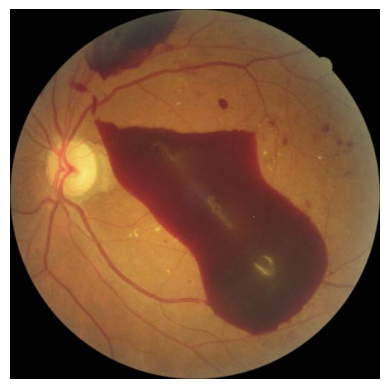
\includegraphics[width=\textwidth]{image-1.png}
    \end{subfigure}
    \hspace{5mm}
    \begin{subfigure}[b]{0.2\textwidth}
        \centering
        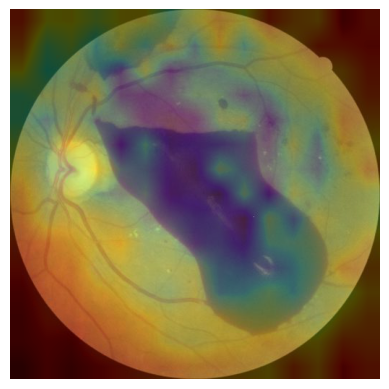
\includegraphics[width=\textwidth]{cbam-heatmap-1.png}
    \end{subfigure}
    \hspace{5mm}
    \begin{subfigure}[b]{0.2\textwidth}
        \raggedright
        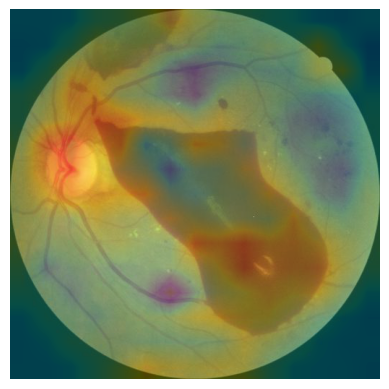
\includegraphics[width=\textwidth]{cabnet-heatmap-1.png}
    \end{subfigure} \\
    \vspace{5mm}
    \begin{subfigure}[b]{0.2\textwidth}
        \raggedleft
        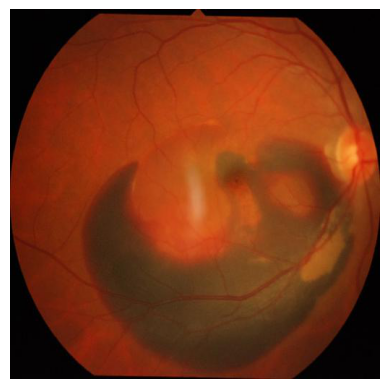
\includegraphics[width=\textwidth]{image-2.png}
    \end{subfigure}
    \hspace{5mm}
    \begin{subfigure}[b]{0.2\textwidth}
        \centering
        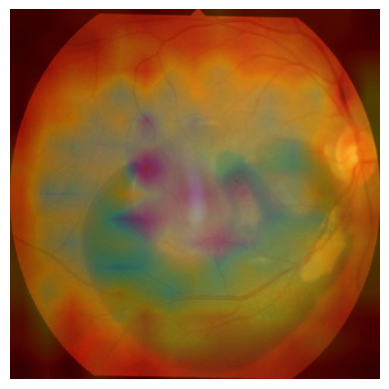
\includegraphics[width=\textwidth]{cbam-heatmap-2.png}
    \end{subfigure}
    \hspace{5mm}
    \begin{subfigure}[b]{0.2\textwidth}
        \raggedright
        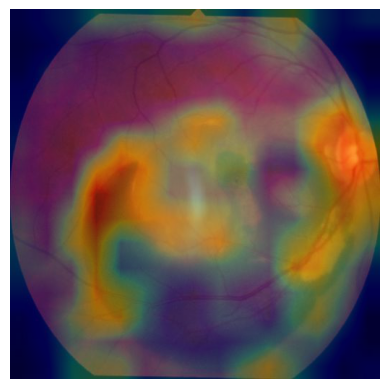
\includegraphics[width=\textwidth]{cabnet-heatmap-2.png}
    \end{subfigure} \\
    \vspace{5mm}
    \begin{subfigure}[b]{0.2\textwidth}
        \raggedleft
        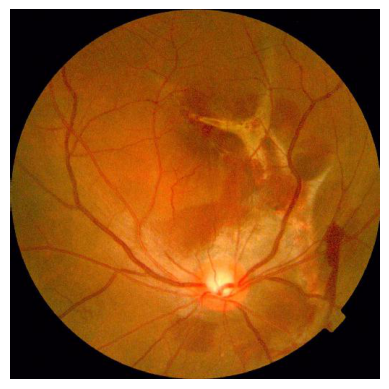
\includegraphics[width=\textwidth]{image-3.png}
        \caption{原始图片}
    \end{subfigure}
    \hspace{5mm}
    \begin{subfigure}[b]{0.2\textwidth}
        \centering
        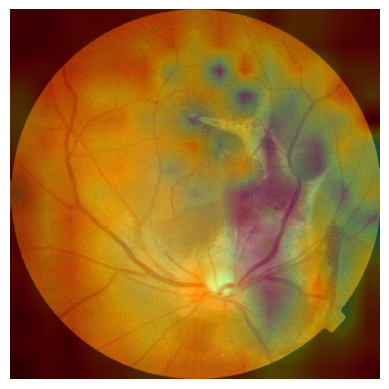
\includegraphics[width=\textwidth]{cbam-heatmap-3.png}
        \caption{CBAM 结果}
    \end{subfigure}
    \hspace{5mm}
    \begin{subfigure}[b]{0.2\textwidth}
        \raggedright
        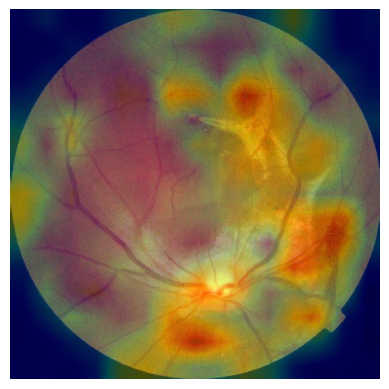
\includegraphics[width=\textwidth]{cabnet-heatmap-3.png}
        \caption{GAB+CAB 结果}
    \end{subfigure}
    
    \caption{原始图片、CBAM 及 CABNet 注意力机制得到的 Heatmap}
    \label{fig:attention_cbam_cabnet}
\end{figure}

  从图 \ref{fig:attention_cbam_cabnet} 中可以发现 CABNet 所得到的 attention 的结果与图片中发生病变的区域更加吻合,而 CBAM 则几乎没有关注原始图像中的有关部分。可见 CABNet 中 GAB 和 CAB 的机制的确是有着巨大作用的,而实验中的 CBAM 模块似乎并没有起到很大作用。与 CBAM 相比,使用 Patch Embedding 作为 Backbone 加上 CBAM 模块所得到的权重似乎更符合原始图片中的病变情况(图 \ref{fig:spatial_attention}),或许 ConvNeXt 所做的特征提取对 CBAM 的效果存在着影响。

\section{混淆矩阵及分类精度}

\begin{figure}[H]
    \centering
    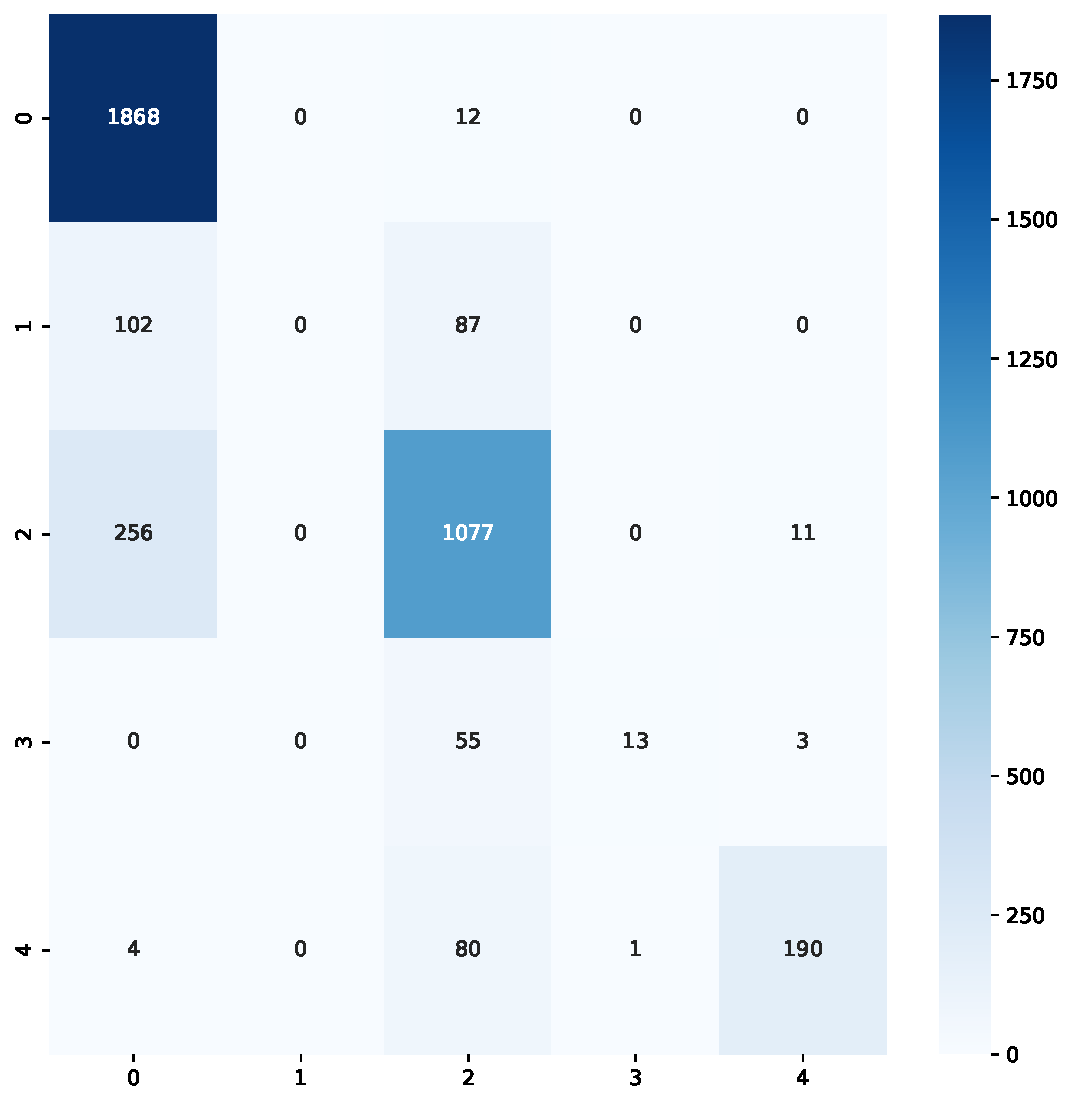
\includegraphics[width=0.5\linewidth]{confusion_matrix.pdf}
    \caption{ConvNeXt + CBAM + ConvMixer 在 test 集上得到的混淆矩阵生成的 Heatmap}
    \label{fig:confmat}
\end{figure}

  如图 \ref{fig:confmat} 所得到的混淆矩阵,第一类(Mild DR)被分到了第零类(No DR)和第二类(Moderate DR)。而第三类也存在着被误分为第二类的情况,猜想这种情况存在着两种可能的原因:
  \begin{enumerate}
      \item 测试集上样本分布与训练集差距较大,第一类的数量所占比例更少;
      \item 模型本身也不能很好地对前四种进行分类。
  \end{enumerate}
  
  尽管实验中所得得到的 Kappa 系数表明模型具有较好的分类精度,但是在各个类别实际的分类表现上模型仍然存在着不足。
  

\end{appendices}


\end{document}
 